\chapter{系统建模和形式化描述}

本章旨在为分布式数据库的一致性模型建立统一的形式化描述框架。
首先，本章阐述了分布式环境下进行一致性建模的必要性，分析了网络延迟和节点故障对事务执行结果的影响。
其次，本章定义了事务、操作、日志和快照等基本概念，引入可见性关系（VIS）和仲裁关系（AR）两个核心二元关系，构建了 $(\text{VIS}, \text{AR})$ 规约框架。
然后，本章提出了六条一致性公理，分别为内部一致性、外部一致性、传递可见性、前缀一致性、无冲突和完全可见性，并给出了形式化定义。
最后，本章基于这些公理定义了六个隔离级别，从弱到强依次为读原子性（Read Atomic，RA）、因果一致性（Causal Consistency，CC）、并发快照隔离（Parallel Snapshot Isolation，PSI）、
前缀一致性（Prefix Consistency，PC）、快照隔离（Snapshot Isolation，SI）和可串行化（Serialisability，SER），
并分析了各级别之间的偏序关系及其能够防止或允许的异常类型。


\section{一致化建模的必要性}
理想情况下，我们希望事务执行结果具有原子性（Atomicity）和隔离性（Isolation）的保证——每个事务都应成为一个独立、不可分割的工作单位，不受任何另一事务干扰。最直接的做法是：使数据库在事务执行时对涉及的数据进行全局锁定，仅允许一个事务进行修改。然而，这种做法对性能的伤害极大——数据库无法处理高并发请求，实际上根本不可用。一般的数据库具有可串行化的隔离级别，尽管在此级别下，为了提高数据库系统的性能，数据库事务依然是支持并发执行的，只是数据库通过加锁等机制，确保事务的执行结果与某个串行执行顺序等价，从而避免数据不一致异常的发生。

一致性模型不一定是越强越好。越强的一致性，需要更多协调、更多同步、更多等待、更高延迟、更低吞吐；越弱的一致性，允许更多异步、更多本地优化、更高并发、更低延迟，但异常更多。性能和更强的一致性站在天平的两端，我们必须做出权衡（trade-offs）。 为了支持事务并发（Concurrency），数据库必须向高一致性妥协，所谓接受一些数据不一致异常（Anomalies）的发生。数据库选择上可接受的异常种类决定了其一致性模型（Consistency Model）。不同的一致性模型对事务执行时施加的约束不同，事务在执行前和在执行后都必须符合该一致性模型的要求。

分布式数据库作为一种分布式系统，其各个节点通常分布在不同的物理节点上，通过网络进行通信。
网络通信的延迟和故障往往是不可避免的，这导致分布式数据库除了考虑如单点数据库在不同隔离级别下的异常外，还需要考虑网络延迟和故障带来的异常。

考虑以下情形：
\begin{equation}
    \begin{aligned}
        \operatorname{txn_1}    & \{\operatorname{write}(x, \text{post}); \operatorname{write}(y, \text{null})\} \\
        \| \operatorname{txn_2} & \{u=\operatorname{read}(x) ; \operatorname{write}(y, \text{comment})\}         \\
        \| \operatorname{txn_3} & \{v=\operatorname{read}(x) ; w=\operatorname{read}(y)\}
    \end{aligned}
\end{equation}
其中 $x$ 和 $y$ 是两个数据项，$u$、$v$、$w$ 为读操作的结果。在串行执行（$txn_1$ 提交后 $txn_2$ 执行，$txn_2$ 提交后 $txn_3$ 执行）假设下，不考虑分布式情景，仅在本地数据库执行，应有 $u=\text{post}$、$v=\text{post}$、$w=\text{comment}$。
但在分布式环境中，网络延迟会导致更新的异步传播。例如，$txn_1$ 因网络故障而延迟到达 $txn_3$ 节点，但已到达 $txn_2$ 节点，导致 $txn_3$ 读到的是 $u=\text{post}$、$v=\text{null}$、$w=\text{comment}$ 的不一致状态。类似地，若 $txn_1$ 完全延迟到 $txn_2$ 之后才到达 $txn_3$ 节点，$txn_3$ 可能只看到 $v=\text{null}$、$w=\text{comment}$ 的部分更新。

一致性模型的定义，规定了在分布式环境下允许出现的数据不一致类型。这份协议并非抽象约定，而是对并发操作、副本同步、故障恢复、分片协作、事务执行等所有可能导致数据可见性异常的场景，做出的形式化、可验证、可推理的行为约束。它精确界定了如：
\begin{itemize}
    \item 写操作完成后，其他客户端、其他节点、其他事务在何种条件下可以观测到该写操作；
    \item 多个操作（来自不同客户端、不同分片、不同副本）在全局时序中如何排序；
    \item 哪些异常现象（脏读、不可重复读、幻读、写偏序、副本滞后、读撕裂、部分提交）是被允许的，哪些是被严格禁止的；
    \item \dots
\end{itemize}

一致性模型的定义，是数据库和应用程序开发者之间的契约，它让数据库底层的复杂实现和上层应用逻辑解耦。开发者可以根据应用需求选择合适的一致性模型，数据库系统则负责在该模型下正确、高效地执行事务，而不需要理解数据库是如何运行的。这种契约关系是分布式系统可规模化、可维护、可替换、可升级的基础。如果没有这份契约，每个版本的数据库行为可能不同；每次故障 / 切换可能带来不可预期的读 / 写结果 \dots 导致应用无法编写稳定、可移植、可验证的逻辑。


\section{基本建模}
以全局视角看，考虑到事务在提交时间维度上存在先后关系，我们用符号 \History（History）表示全局事务的执行历史，它是一系列事务（Transaction，记为 \Txc 或 \Txc[x]）的有序集合。\History 还需要标注隔离级别（Isolation Level），本文涉及六个隔离级别，从高到低分别为可串行化（Serialisability，SER）、快照隔离（Snapshot Isolation，SI）、前缀一致性（Prefix Consistency，PC）、并发快照隔离（Parallel Snapshot Isolation，PSI）、因果一致性（Causal Consistency，CC）和读原子性（Read Atomic，RA）\cite{Schultz2015}，我们将在后文中详细介绍。一个事务 \Txc 则是一系列操作（Operation）的执行序列。我们的研究目标是键值数据库，不考虑复杂的谓词操作，具体操作可抽象为以下几种类型：
\begin{itemize}
    \item \OpStart：事务开始操作，标志着一个新事务的启动。
    \item \OpCommit：事务提交操作，表示事务成功完成并将其更新持久化。
    \item \OpAbort：事务中止操作，表示事务执行失败，所有更改被回滚。
    \item \OpRead[k][v]：读操作，表示读取键 $k$ 的值，期望读取结果为 $v$。
    \item \OpWrite[k][v]：写操作，表示将键 $k$ 的值设置为 $v$。
\end{itemize}
其中，\OpRead 和 \OpWrite 操作的对象是键 $k$，所有键的集合记为 \Keys。在复制型分布式数据库中，\OpReceive 操作对于理解节点间的数据同步至关重要：当一个事务在某个节点提交后，其更新需要通过网络传播到其他节点，其他节点通过 \OpReceive 操作接收并应用这些更新。

快照（Snapshot，记为 \Snapshot）表示某一时刻数据库的一致性状态。具体来说，快照是当前节点执行完成一个完整事务后的状态，无论该事务是本地提交的还是通过 \OpReceive 从其他节点接收的。在快照状态下，系统没有事务正在执行。

在给出形式化表达时，我们使用二元组来表示序列概念。以事务 \Txc 为例，一个事务 \Txc 是一个二元组 $(O, po)$，其中 $O \subseteq Op$ 是该事务包含的操作集合，$Op$ 为所有可能操作的有限非空集合。$po \subseteq O \times O$ 称为程序顺序（program order），是一个严格全序关系，表示事务内操作的执行顺序。同样的，\History 也有类似的定义方式，其中的$SO$ 也是一个严格全序关系，表示事务之间的执行顺序。

以上概念的形式化表达如下：
\begin{equation}
    \begin{aligned}
        \mathcal{K} & = \{ x, y, \ldots\}, \quad \mathcal{V} = \{ \bot ,1, 2, \ldots, n \}                                                                         \\
        Op          & = \{ \text{start}, \text{commit}, \text{abort} \} \cup \{ \text{read}(k, v), \text{write}(k, v) \mid k \in \mathcal{K}, v \in \mathcal{V} \} \\
        T           & = (O, po), O \subseteq Op, \quad  po \subseteq O \times O                                                                                    \\
        \mathcal{H} & = (\mathcal{T}, SO, level), \quad \mathcal{T} = \{T_1, T_2, \ldots, T_n\},                                                                   \\
                    & \quad SO \subseteq \mathcal{T} \times \mathcal{T}, \quad level \in \{\text{SER}, \text{SI}, \text{PC}, \text{PSI}, \text{CC}, \text{RA}\}    \\
        S           & : \mathcal{K} \rightharpoonup \mathcal{V},  S(k) = \bot \text{ if } k \notin \text{dom}(S)
    \end{aligned}
\end{equation}
其中，$\mathcal{K}$ 为键的集合，$\mathcal{V}$ 为值的集合（$\bot$ 表示空值），
$SO$ 为会话顺序（session order），表示同一会话内事务的执行顺序，
$S$ 为快照函数，将键映射到其对应的值。

此外，还有两个辅助运算符用于求得事务的读集合和写集合：
\begin{equation}
    \begin{aligned}
        \operatorname{RSet}(T) & = \{ k \in \mathcal{K} \mid \exists O_i = \text{read}(k, \cdot) \in T, \forall j < i, O_j \neq \text{write}(k, \cdot) \} \\
        \operatorname{WSet}(T) & = \{ k \in \mathcal{K} \mid \exists O \in T, O = \text{write}(k, v) \}
    \end{aligned}
\end{equation}
其中，$\operatorname{RSet}(T)$ 表示事务 $T$ 的读集合，即在本事务内被读取且在读取前未被本事务写入的键的集合；$\operatorname{WSet}(T)$ 表示事务 $T$ 的写集合，即被本事务写入的键的集合。

当两个事务的写集合交集不为空，即 $\operatorname{WSet}(T_1) \cap \operatorname{WSet}(T_2) \neq \emptyset$ 时，称这两个事务存在写冲突（write-conflict），记为 $T_1 \bowtie T_2$。

\subsection{VIS 和 AR 关系}
由于事务的处理结果是原子化的，而多个事务的处理是并发的，因此描述事务隔离级别的关键在于描述任意两个事务之间的关系。这些关系是事务集合笛卡尔积 $\mathcal{T} \times \mathcal{T}$ 的子集。我们重点考虑两个核心关系：$\text{VIS}, \text{AR} \subseteq \mathcal{T} \times \mathcal{T}$。

可见性关系（Visibility Relation）$\text{VIS} \subseteq \mathcal{T} \times \mathcal{T}$ 定义了一个事务的执行结果对另一个事务是否可见。
直观地说，如果 $(T_1, T_2) \in \text{VIS}$，也就是 $T_1 \xrightarrow{\text{VIS}} T_2$，则表示事务 $T_1$ 的所有写操作对事务 $T_2$ 可见，即 $T_2$ 在执行读操作时能够读取到 $T_1$ 写入的值。$\text{VIS}$ 是一个无环的偏序关系，即不存在 $T_1 \xrightarrow{\text{VIS}} T_2 \xrightarrow{\text{VIS}} T_1$ 的情况。可见性关系决定了事务读取数据时所看到的快照状态，是理解事务隔离级别的核心概念之一。从另一个角度看，两个事务之间不存在可见性关系意味着它们是并发的。

仲裁关系（Arbitration Relation）$\text{AR} \subseteq \mathcal{T} \times \mathcal{T}$ 定义了事务之间写操作的全局顺序。当 $(T_1, T_2) \in \text{AR}$，即 $T_1 \xrightarrow{\text{AR}} T_2$ 时，表示事务 $T_1$ 的写操作在逻辑上先于事务 $T_2$ 的写操作，换言之，$T_2$ 的写入结果会覆盖 $T_1$ 对相同键的写入。$\text{AR}$ 是一个全序关系，即对于任意两个事务 $T_1$ 和 $T_2$，要么 $T_1 \xrightarrow{\text{AR}} T_2$，要么 $T_2 \xrightarrow{\text{AR}} T_1$。仲裁关系确定了并发写操作的最终顺序，解决了写冲突问题。


在进一步讨论这两个关系之前，我们需要明确一个重要的性质：$\text{VIS} \subseteq \text{AR}$，即可见性关系是仲裁关系的子集。这个性质并非偶然，而是保证数据库系统正确性的必要条件。

直观地理解,如果事务$T_1$的写入对事务$T_2$可见(即$T_1 \xrightarrow{\text{VIS}} T_2$),那么在逻辑上,$T_1$的写操作必然先于$T_2$的写操作被系统接受(即$T_1 \xrightarrow{\text{AR}} T_2$)。这是因为,$T_2$能够读取到$T_1$的写入结果,说明$T_1$已经成功提交,并且其写入的值没有被后续的其他事务覆盖。因此,在全局的写操作顺序中,$T_1$必然排在$T_2$之前。

从另一个角度看，$\text{VIS}$是一个偏序关系（partial order），它描述了事务之间已经确定的因果依赖关系。而$\text{AR}$是一个全序关系（total order），它为所有事务的写操作定义了一个全局的先后顺序。$\text{AR}$的作用是在$\text{VIS}$的基础上进行扩展：对于已经存在$\text{VIS}$关系的事务对，$\text{AR}$必须遵守这个既定的顺序；对于没有$\text{VIS}$关系的并发事务，$\text{AR}$需要"仲裁"出一个确定的顺序，以解决写冲突。

在实际的数据库系统实现中,$\text{AR}$通常通过时间戳(Timestamps)机制来实现。如果$T_1 \xrightarrow{\text{VIS}} T_2$,意味着$T_2$在执行时已经观察到了$T_1$的更新,或者$T_2$是在$T_1$提交之后才开始执行的。因此,$T_2$获取的时间戳必然晚于$T_1$的时间戳,从而保证$T_1 \xrightarrow{\text{AR}} T_2$。

这个性质$\text{VIS} \subseteq \text{AR}$的重要意义在于：
\begin{itemize}
    \item \textbf{保证因果一致性}：如果一个事务观察到了另一个事务的结果，那么在全局顺序中，前者必须排在后者之前，这确保了因果关系的正确传递。
    \item \textbf{确保数据正确覆盖}：对于有可见性关系的事务，后来者的写入应当覆盖前者的写入，避免出现"时光倒流"的异常情况。
    \item \textbf{提供一致性基础}：这个性质是定义和实现各种隔离级别的基础，不同的隔离级别可以在此基础上施加额外的约束。
\end{itemize}

因此，$\text{VIS} \subseteq \text{AR}$不仅是一个数学性质，更是分布式数据库系统保证数据一致性和正确性的核心机制。

这两个关系共同构成了$(\text{VIS}, \text{AR})$规约框架，为分布式数据库的一致性模型提供了统一的形式化描述基础。通过对VIS和AR关系施加不同的约束条件，可以精确地刻画不同隔离级别的语义。例如，在可串行化（Serializable）隔离级别下，$\text{VIS}$和$\text{AR}$系需要满足严格的约束，保证事务的执行结果等价于某个串行执行顺序；而在较弱的隔离级别下，这些约束可以适当放松，从而允许更多的并发执行，提高系统性能。

此外，我们约定 $\operatorname{VIS^{-1}}(T)$ 表示对事务 $T$ 可见的所有事务的集合，即 $\operatorname{VIS^{-1}}(T) = \{ T' \in \mathcal{T} \mid T' \xrightarrow{\text{VIS}} T \}$。其他关系的逆集合也做类似约定。我们还定义 $\operatorname{WriteTx}_k$ 表示对键 $k$ 有写操作的事务集合，并用 $T \Vdash \operatorname{op}$ 表示事务 $T$ 包含操作 $\operatorname{op}$。

基于以上提供的符号，我们可以定义抽象执行（Abstract Execution）是一个三元组$\mathcal{X} = (\mathcal{H}, \text{VIS}, \text{AR})$。

\section{一致性公理}
基于上述符号以及 $\text{VIS}$、$\text{AR}$ 的定义，我们可以定义一致性公理。

所有一致性模型必须遵守以下两个基础公理：
\begin{itemize}
    \item \textbf{Int（内部一致性公理，Internal Consistency）}：
          内部一致性公理确保事务内部的读写行为符合串行语义。
          例如，一个事务如果先写了某个对象再读该对象，
          必须能读到自己刚写入的值。
          这条公理保证了单事务视角的逻辑正确性。
    \item \textbf{Ext（外部一致性公理，External Consistency）}：
          外部一致性公理定义了事务如何读取其他事务写入的值。
          它规定，对于本事务未写入过的对象的读取（外部读取），
          其值取决于所有对它可见的事务中，在 AR 顺序下最新的那个事务写入的值。
          这条公理用于防止断裂读取（Fractured Reads）和脏读（Dirty Reads）。
\end{itemize}

除此之外，还有四个额外公理可用于进一步刻画一致性模型的语义：
\begin{itemize}
    \item \textbf{TransVis（传递可见性，Transitive Visibility）}：
          传递可见性公理确保如果事务 $T_1$ 对事务 $T_2$ 可见，
          而 $T_2$ 又对事务 $T_3$ 可见，
          那么 $T_1$ 对 $T_3$ 也必须可见。
          这条公理用于防止因果违例（Causality Violation）。
          例如，Alice 发帖，Bob 看到后评论。
          如果 Charlie 看到了 Bob 的评论，根据传递性，Charlie 也必须能看到 Alice 的原帖。
    \item \textbf{Prefix（前缀一致性，Prefix Consistency，PC）}：
          前缀一致性公理确保如果事务 $T_2$ 对 $T_1$ 可见，
          那么在 $\text{AR}$ 顺序下排在 $T_2$ 之前的所有事务也必须对 $T_1$ 可见。
          换言之，事务所看到的历史必须是一个完整的、没有空洞的前缀（Snapshot）。
          这条公理用于防止长分叉（Long Forks），
          即防止两个并发事务各自看到不同的、不兼容的历史版本。
    \item \textbf{NoConflict（无冲突）}：
          无冲突公理确保如果两个事务存在写冲突，
          则它们之间必须存在可见性关系，不能彼此并发而互不可见。
          这条公理用于防止丢失更新（Lost Update），
          即防止某个事务的更新被另一个并发事务直接覆盖。
    \item \textbf{TotalVis（完全可见性，Total Visibility）}：
          完全可见性公理要求 $\text{VIS}$ 关系必须是一个全序关系，
          即对于任意两个事务 $T_1$ 和 $T_2$，
          要么 $T_1 \xrightarrow{\text{VIS}} T_2$，要么 $T_2 \xrightarrow{\text{VIS}} T_1$。
          这意味着所有事务都在一条单一的时间线上，
          每个事务都能看到它之前的所有事务。
          这是最强的公理。
\end{itemize}
其中，TransVis 和 Prefix 两条公理是对 $\text{VIS}$ 关系的限制和强化，而 NoConflict 和 TotalVis 两条公理主要聚焦于写冲突的解决方案。

以上公理的形式化表达如下：
\begin{equation}
    \label{eq:consistency}
    \begin{aligned}
        \mathsf{Int}(T)        & \equiv \forall r \in O.\ \forall x, v.\ \bigl(r = \operatorname{read}(x, v) \land po_x^{-1}(r) \neq \emptyset\bigr)                                                                                   \\
                               & \qquad\Rightarrow \max\nolimits_{po}\bigl(po_x^{-1}(r)\bigr) = \operatorname{write}(x, v),                                                                                                            \\[0.4em]
        \mathsf{Ext}(T)        & \equiv \forall x, v.\ T \Vdash \operatorname{read}(x, v) \Rightarrow \max\nolimits_{\text{AR}}\bigl(\operatorname{VIS^{-1}}(T) \cap \operatorname{WriteTx}_x\bigr) \Vdash \operatorname{write}(x, v), \\[0.4em]
        \mathsf{TransVis}(T)   & \equiv \forall T', S \in \mathcal{T}.\ T' \xrightarrow{\text{VIS}} S \land S \xrightarrow{\text{VIS}} T \Rightarrow T' \xrightarrow{\text{VIS}} T,                                                    \\[0.4em]
        \mathsf{Prefix}(T)     & \equiv \forall T', S \in \mathcal{T}.\ T' \xrightarrow{\text{AR}} S \land S \xrightarrow{\text{VIS}} T \Rightarrow T' \xrightarrow{\text{VIS}} T,                                                     \\[0.4em]
        \mathsf{NoConflict}(T) & \equiv \forall T' \in \mathcal{T}.\ T' \bowtie T \land T' \xrightarrow{\text{AR}} T \Rightarrow T' \xrightarrow{\text{VIS}} T,                                                                        \\[0.4em]
        \mathsf{TotalVis}(T)   & \equiv \forall T' \in \mathcal{T}.\ T' \xrightarrow{\text{AR}} T \Rightarrow T' \xrightarrow{\text{VIS}} T.
    \end{aligned}
\end{equation}
其中，$po_x^{-1}(r)$ 表示在程序顺序 $po$ 下排在读操作 $r$ 之前且操作对象为键 $x$ 的所有操作的集合，$\max_{po}$ 表示在程序顺序下取最后一个操作，$\max_{\text{AR}}$ 表示在仲裁顺序下取最新的事务。

\section{隔离级别}
基于上述一致性公理的定义，接下来我们讨论各个隔离级别的特点。为了在一致性、可扩展性和可用性之间取得平衡，现代数据库系统提供了一系列不同强度的隔离级别。这些级别根据其提供的可见性保证和所能防止的异常现象，构成了一个从最弱的“原子读”到最强的“可串行化”的层级体系。
\\

\noindent\textbf{读原子性（Read Atomic，RA）}是最弱的一致性级别，仅满足 $\mathsf{Int}$ 和 $\mathsf{Ext}$ 两个公理。它只保证事务的更新以原子方式对其他事务可见，即要么看到一个事务的全部写入，要么完全看不到该事务。RA 不对事务之间的可见性关系施加额外约束，因此几乎所有其他异常都可能发生。例如图~3(a) 中的因果违背（Causality Violation），$T_2$ 能够看到 $T_1$ 的写入，$T_3$ 能够看到 $T_2$ 的写入，但 $T_3$ 却看不到 $T_1$ 对同一对象的更新，打破了直观上的因果链。

\noindent\textbf{因果一致性（Causal Consistency，CC）}在读原子性的基础上增加了 $\mathsf{TransVis}$ 公理，要求可见性关系 VIS 必须具有传递性。也就是说，如果 $T_3$ 看到了 $T_2$，而 $T_2$ 又看到了 $T_1$，那么 $T_3$ 必须也能看到 $T_1$。因此 CC 能够消除因果违背异常。但由于 CC 并不禁止对同一对象的并发写，丢失更新（Lost Update）异常仍然被允许。

\noindent\textbf{并发快照隔离（Parallel Snapshot Isolation，PSI）}在因果一致性的基础上增加了 $\mathsf{NoConflict}$ 公理。该公理要求对同一对象进行写入的两个事务不能彼此并发而互不可见，它们之间必须通过 VIS 确定先后顺序。直观地说，并发写冲突必须被仲裁，不能惄无声息地丢掉某个更新。因此 PSI 能够排除丢失更新异常。不过，PSI 仍允许不同事务在不同节点上看到不一致的历史前缀，从而产生长分叉（Long Fork）异常。

\noindent\textbf{前缀一致性（Prefix Consistency，PC）}从另一个维度增强因果一致性。它采用 $\mathsf{Prefix}$ 公理来约束可见历史，该公理蕴含了 $\mathsf{TransVis}$，要求如果事务 $T_1$ 看到了 $T_2$，那么在 AR 顺序中排在 $T_2$ 之前的所有事务都必须对 $T_1$ 可见。换言之，每个事务所看到的历史必须是全局 AR 顺序的一段前缀。因此，长分叉异常在 PC 下会被禁止。但由于 PC 并不禁止在同一快照上对不同对象进行并发写入，写偏斜（Write Skew）异常在 PC 中仍可能发生。

\noindent\textbf{快照隔离（Snapshot Isolation，SI）}可看作并发快照隔离与前缀一致性的合流点。它一方面继承了 $\mathsf{Prefix}$，要求所有事务在 AR 序列的某个前缀上执行；另一方面继承了 $\mathsf{NoConflict}$，禁止对同一对象的并发写冲突。因此，SI 同时防止了丢失更新和长分叉两类异常。SI 在一致性和性能之间取得了较好的平衡，因此被许多数据库系统支持或采用。常见数据库系统都有类似的隔离级别实现。然而，由于 SI 仍允许事务在同一快照上对不同对象进行更新，写偏斜异常仍然可能出现。

\noindent\textbf{可串行化（Serialisability，SER）}通过 $\mathsf{TotalVis}$ 公理将可见性关系强化为全序关系。对于任意两个事务 $T_1$ 和 $T_2$，要么 $T_1 \xrightarrow{\text{VIS}} T_2$，要么 $T_2 \xrightarrow{\text{VIS}} T_1$，不再允许它们在抽象执行层面真正并发。从结果上看，所有事务的执行效果等价于按照某个串行顺序依次执行。因此，SER 排除了所有前述异常，包括写偏斜，是图~\ref{fig:isolevels} 中最强的一致性级别。SER 提供了最直观的编程模型，开发者可以假设每个事务是在完全隔离的环境中执行的，无需考虑复杂的并发场景。但其代价是较高的性能开销，因为系统需要通过加锁或乐观并发控制等机制来确保事务的串行化执行。可以补充的是，因为 $VIS \subseteq AR$，强调 VIS 上的全序关系，也是强调 AR 上的全序关系。

表~\ref{tab:consistency-models} 从弱一致性级别到强一致性级别，列出了每个隔离级别需要满足的公理以及能够防止或允许的异常。表中 $\checkmark$ 表示该隔离级别允许该异常发生，$\times$ 表示能够防止该异常。
\begin{table}[htbp]
    \centering
    \caption{一致性模型及其所满足的公理与异常}
    \label{tab:consistency-models}
    \small
    \setlength{\tabcolsep}{4pt} % 减小列间距
    \begin{tabular}{c l c c c c c}
        \hline
        $\Phi$ & Axioms                                            & \makecell{Fractured                                              \\reads} & \makecell{Causality\\violation} & \makecell{Lost\\update} & \makecell{Long\\fork} & \makecell{Write\\skew} \\
        \hline
        RA     & $\mathsf{Int},\ \mathsf{Ext}$
               & $\times$                                          & $\checkmark$        & $\checkmark$ & $\checkmark$ & $\checkmark$ \\
        \midrule
        CC     & $\mathsf{Int},\ \mathsf{Ext},\ \mathsf{TransVis}$
               & $\times$                                          & $\times$            & $\checkmark$ & $\checkmark$ & $\checkmark$ \\
        \midrule
        PSI    & \makecell[l]{$\mathsf{Int},\ \mathsf{Ext},$                                                                          \\$\mathsf{TransVis},\ \mathsf{NoConflict}$}
               & $\times$                                          & $\times$            & $\times$     & $\checkmark$ & $\checkmark$ \\
        \midrule
        PC     & $\mathsf{Int},\ \mathsf{Ext},\ \mathsf{Prefix}$
               & $\times$                                          & $\times$            & $\times$     & $\times$     & $\checkmark$ \\
        \midrule
        SI     & \makecell[l]{$\mathsf{Int},\ \mathsf{Ext},$                                                                          \\$\mathsf{Prefix},\ \mathsf{NoConflict}$}
               & $\times$                                          & $\times$            & $\times$     & $\times$     & $\times$     \\
        \midrule
        SER    & $\mathsf{Int},\ \mathsf{Ext},\ \mathsf{TotalVis}$
               & $\times$                                          & $\times$            & $\times$     & $\times$     & $\times$     \\
        \hline
    \end{tabular}
\end{table}

\begin{figure}[htbp]
    \centering
    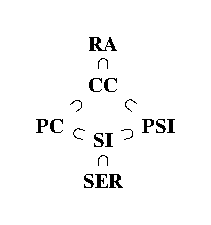
\includegraphics[width=0.4\textwidth]{figures/isolevels.pdf}
    \caption{隔离级别间的偏序关系}
    \label{fig:isolevels}
\end{figure}



从图~\ref{fig:isolevels} 和表~\ref{tab:consistency-models} 可以看出，本文讨论的六个隔离级别在一致性约束上形成了一条从弱到强的偏序链。




